\section*{Caracterização geral da simulação}

%sistemas
\noindent
Este \textit{Call center} tem dois sistemas separados:
\begin{itemize}
    \item Sistema GP, que atende todas as chamadas e reencaminhada chamadas para o sistema AS se necessário
    \item Sistema AS, que atende as chamadas de carácter específico reencaminhadas pelo sistema GP
\end{itemize}

%parametros
\noindent
Definimos os seguintes parâmetros de funcionamento do \textit{Call center}:
\begin{itemize}
    \item Nº de servidores no sistema GP
    \item Nº de servidores no sistema AS
    \item Tamanho da fila de espera no sistema GP (infinita no sistema AS)
\end{itemize}


%chamadas
\noindent
Sendo esta uma simulação de um \textit{Call center}, duas situações podem acontecer:
\begin{itemize}
    \item 30\% de probabilidade de uma chamada apenas precisar de ser atendida no sistema GP.
    \item 70\% de probabilidade de uma chamada precisar de ser no sistema GP e depois no sistema AS.
\end{itemize}


%eventos
\noindent
Distinguem-se 3 tipos de eventos no sistema:
\begin{itemize}
    \item CHEGADA: Uma chamada que chega a um sistema, sem discriminação do seu tipo.
    \item PARTIDA\_GP: Uma chamada que é atendida no sistema GP e depois sai do sistema.
    \item PARTIDA\_AS: Uma chamada que é atendida no sistema GP e entra no sistema AS / Chamada que é atendida no AS
\end{itemize}

As distinção entre PARTIDA\_GP e PARTIDA\_AS é apenas relevante no sistema GP. No sistema AS, faz-se uma abstração para apenas PARTIDA.

Cada evento tempo um \textit{timestamp} associado.
No evento de \textbf{CHEGADA}, define o momento em que chegou.
Nos de \textbf{PARTIDA}, o momento em que partiu.
Este valores são gerados conforme indicado no guião.
\newline

%listas
\noindent
A \textbf{lista\_eventos\_gp} é uma fila onde serão guardados todos os eventos que chegam ao sistema GP.
A \textbf{lista\_espera\_gp} é uma fila onde serão guardados todos os eventos que estão num determinando momento na fila de espera para serem processados pelo sistema GP.
Um evento é colocado na fila de espera quando todos servidores estão ocupados.
Se a fila estiver cheia, a chamada é considerada como perdida e removida.

A \textbf{lista\_eventos\_as} e a \textbf{lista\_espera\_as} têm a mesma funcionalidade mas para o sistema AS.
Um evento é colocado na fila de espera quando o os servidores estão ocupados.
A fila de espera é infinita, pelo que não haverá chamadas perdidas.

\section*{Descrição do funcionamento do algoritmo}

\begin{figure}[H]
    \centering
    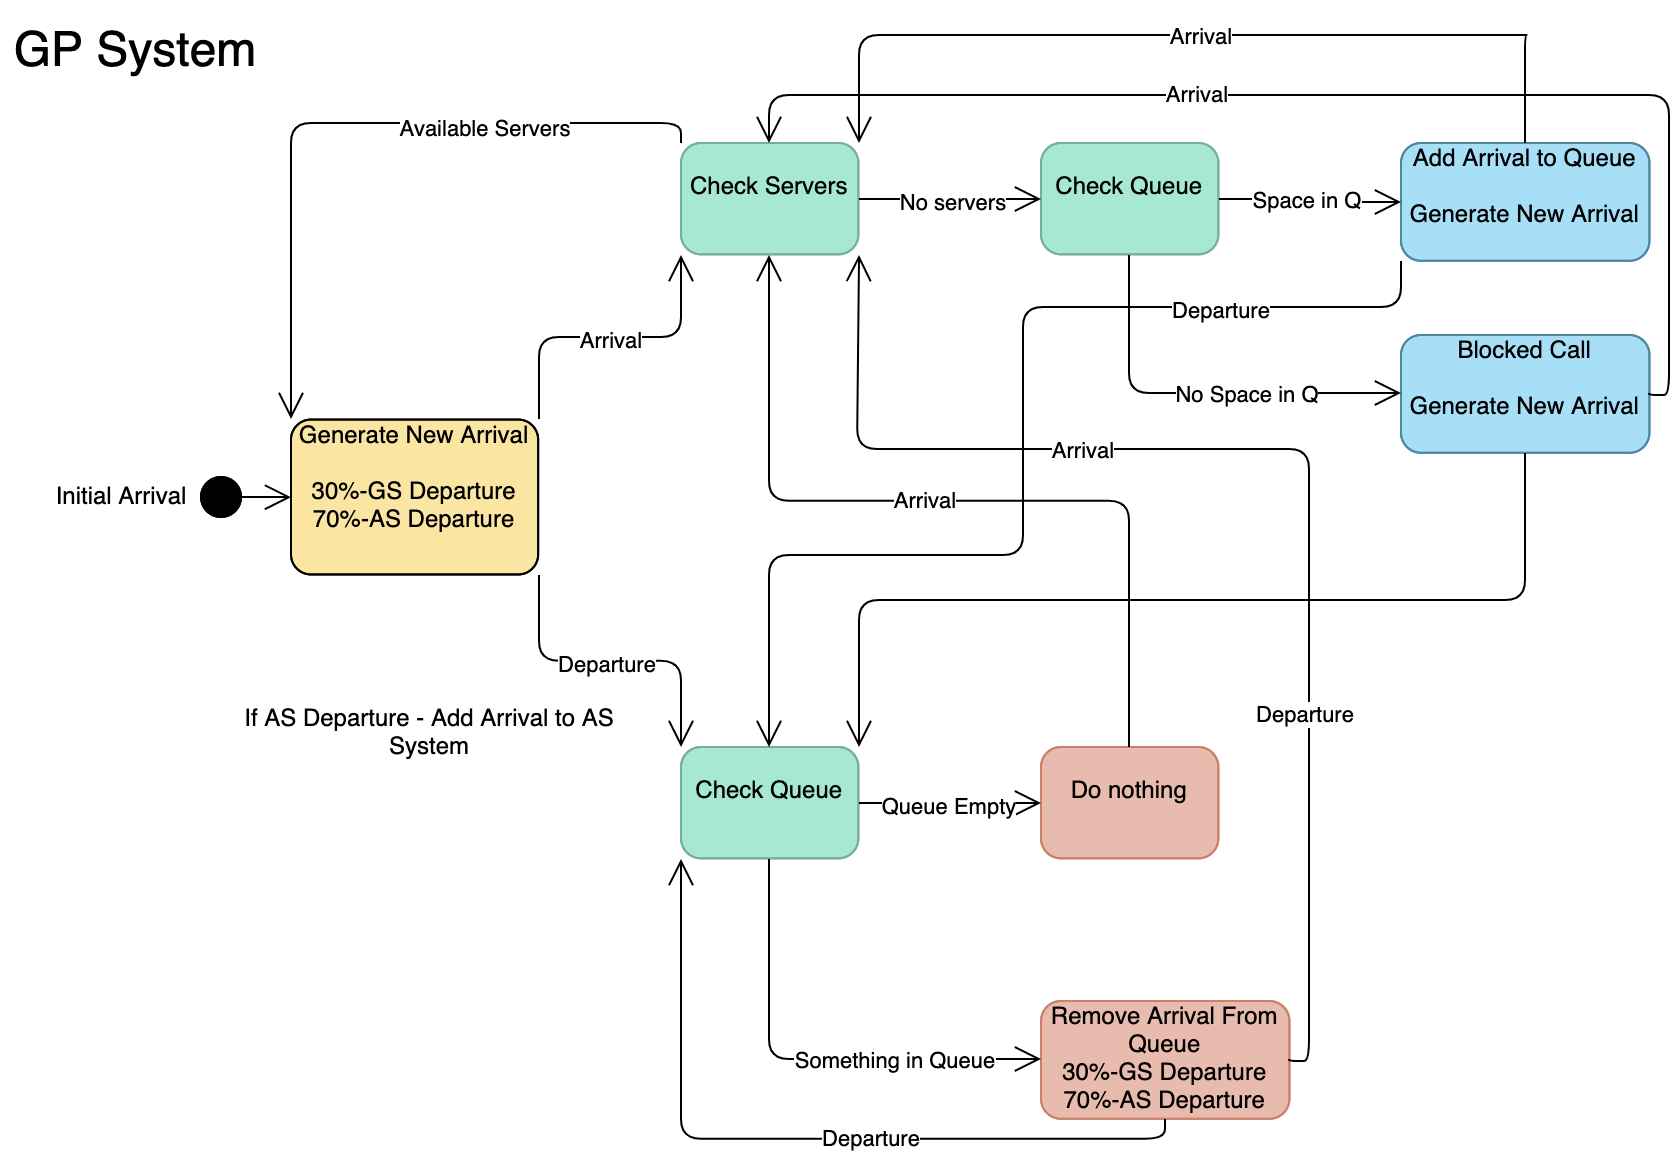
\includegraphics[width=.9\linewidth]{figs/intro/sm_gp.png}
    \caption{Máquina de estados do Sistema General Purpose}
    \label{fig:sm_gp}
\end{figure}

A figura \ref{fig:sm_gp} é uma máquina de estados que representa o algoritmo do \textbf{sistema GP}.
Primeiro verifica-se o tipo de evento que está na \textbf{lista\_eventos\_gp}.

Se o evento for de \textbf{CHEGADA}, verifica-se o estado do sistema.
Se os servidores estivem ocupados, verifica-se a fila de espera.
Se esta estiver livre, esse evento é colocado na \textbf{lista\_espera\_gp}.
Caso contrário é bloqueado.
Novas \textbf{CHEGADAS} são sempre geradas quando se processa uma \textbf{CHEGADA}.

Se o evento for de \textbf{PARTIDA}, verifica-se se há algum evento na \textbf{lista\_espera\_gp}.
Se houver, começa-se imediatamente a processar esse evento, gerando uma nova \textbf{PARTIDA}.
Caso contrário, passa-se para o próximo evento na \textbf{lista\_eventos\_gp}.

Por fim, considera-se que uma \textbf{CHEGADA} é gerada no \textbf{sistema AS} quando é processada uma \textbf{PARTIDA\_AS}.


\noindent
\newline
O princípio de funcionamento do sistema AS é semelhante, ilustrado na figura \ref{fig:sm_as}. Destaca-se alguma diferenças.


As \textbf{CHEGADAS} não são geradas no \textbf{sistema AS}, mas sim no \textbf{sistema GP}, pelo que o sistema pode ficar inativo, algo que não acontece com o \textbf{sistema GP}.
Além disso, não existe a risco de uma chamada ser bloqueada pois a fila é infinita.
A \textbf{lista\_eventos\_as} é constantemente verificada para detetar se alguma chamada foi reencaminhada para ser atendida pela sistema. Quando o sistema fica \textit{idle}, volta a este estado.

As \textbf{PARTIDAS} são geradas também quando uma CHEGADA é processada, no entanto a distribuição temporal é diferente das duas partidas do sistema GP.

\begin{figure}[H]
    \centering
    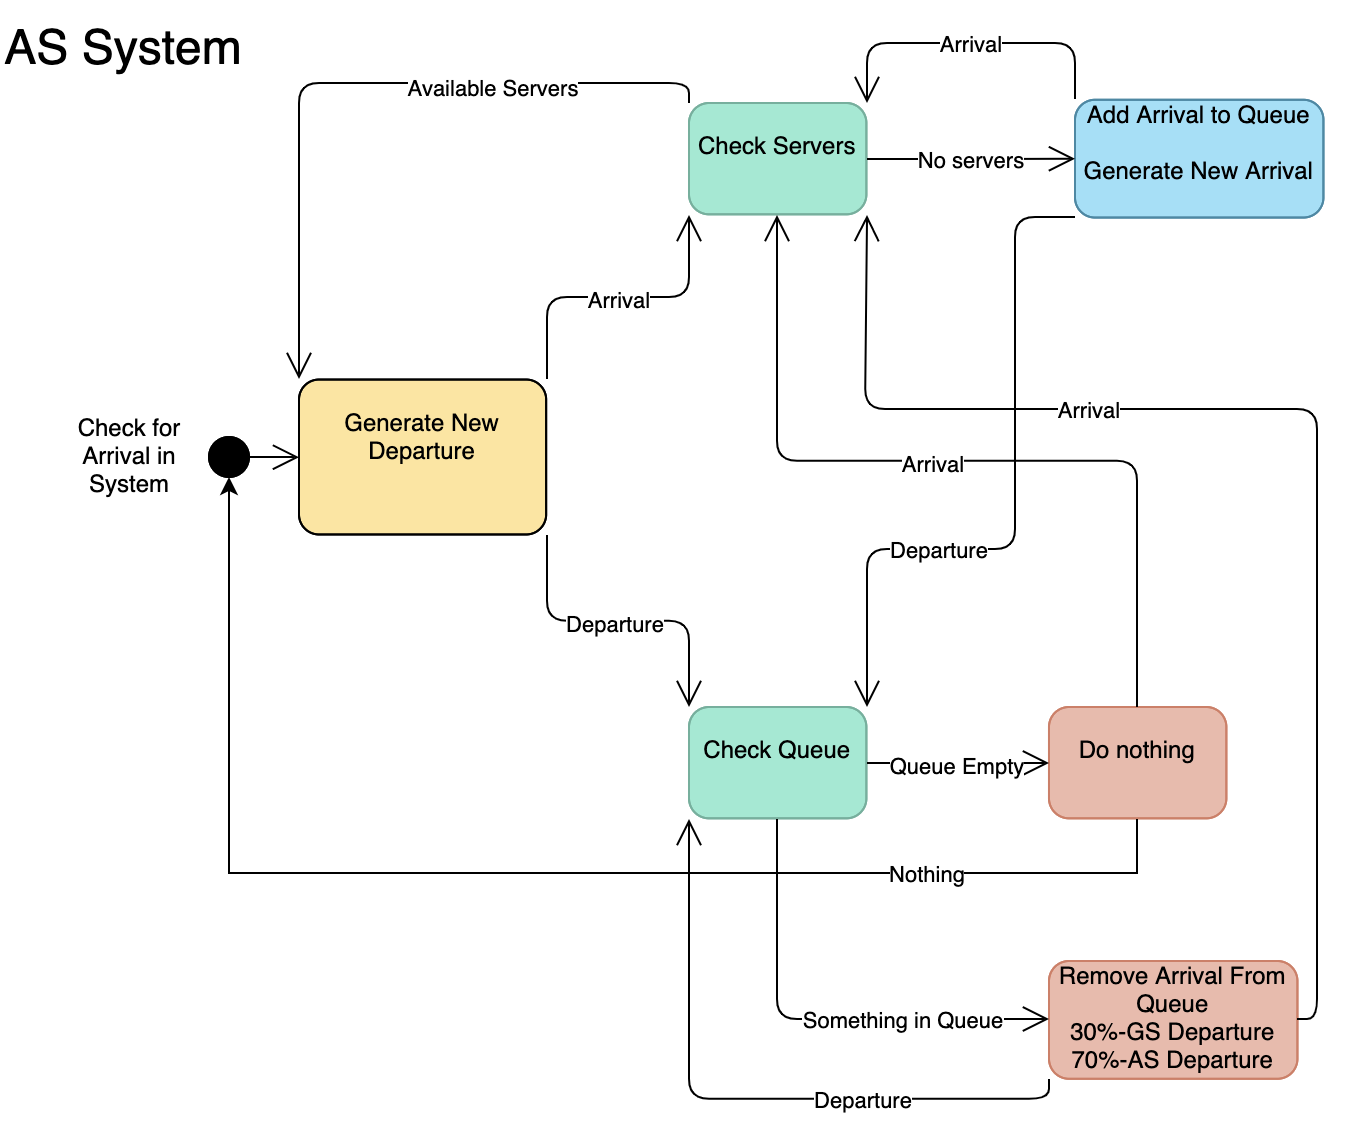
\includegraphics[width=.7\linewidth]{figs/intro/sm_as.png}
    \caption{Máquina de estados do Sistema Area Specific}
    \label{fig:sm_as}
\end{figure}

\section*{Estimativa do tempo de espera}

De forma a puder fornecer uma previsão do tempo de espera a cada chamada que chega, é necessário adotar um algoritmo de \textit{running average}.
Este algoritmo permite o calculo dinâmico da média do tempo de espera a cada chamada que chega, atualizando a cada iteração.

A estimativa do tempo de espera começa a 1. Quando uma chamada chega, duas situações podem acontecer:
\begin{itemize}
    \item Chamada é imediatamente atendida, pelo que o delay é 0 segundos.
    \item Chamada é colocada na fila de espera. O delay é calculado no momento em que a chamada sai da fila de espera.
\end{itemize}

Quando um novo valor de delay é obtido, uma nova média é calculada.
Por exemplo, com um delay de 60 segundos, a nova média será $\frac{0+60}{2}=30s$.
Quando uma nova chamada chegar, a estimativa de tempo de espera apresentada será de 30 segundos.
A cada iteração, este valor é atualizado.
Como este sistema tende para a estabilidade, este valor aproxima-se para um valor constante, que vai fornecer uma previsão mais sólida quantas mais chamadas forem atendidas.


\section*{Resultados da simulação}

De modo a garantir os objetivos de performance mínimos, necessitamos de pelo menos \textbf{4 Servidores GP}, \textbf{2 Servidores AS} e \textbf{Fila de Espera GP de tamanho 2}.
Os seguintes parâmetros foram obtidos:
\begin{center}
    \begin{tabular}{||c|c c||} 
    \hline
    Parâmetro & Mínimo & \textbf{Obtido} \\
    \hline\hline
    Delay Prob & 30\% & \textbf{12.83\%}\\ 
    \hline
    Blocked Prob & 2\% & \textbf{1.35\%}\\
    \hline
    Avrg Delay GS& 30s & \textbf{23.4s}\\
    \hline
    Avrg Delay Total & 60s & \textbf{24s} \\
    \hline
   \end{tabular}
\end{center}

O \textit{Bottleneck} deste sistema é o \textbf{Avrg Delay GS}, que está muito mais próximo do limite do que os restantes parâmetros.
Um relaxamento deste parâmetro para 40 segundo permitia que fosse utilizado apenas 3 servidores GP.

Com estes parâmetros, foram gerados histogramas que representam a distribuição dos atrasos e dos erros de previsão.

\begin{figure}[H]
    \centering
    \begin{subfigure}[b]{0.49\textwidth}
        \centering
    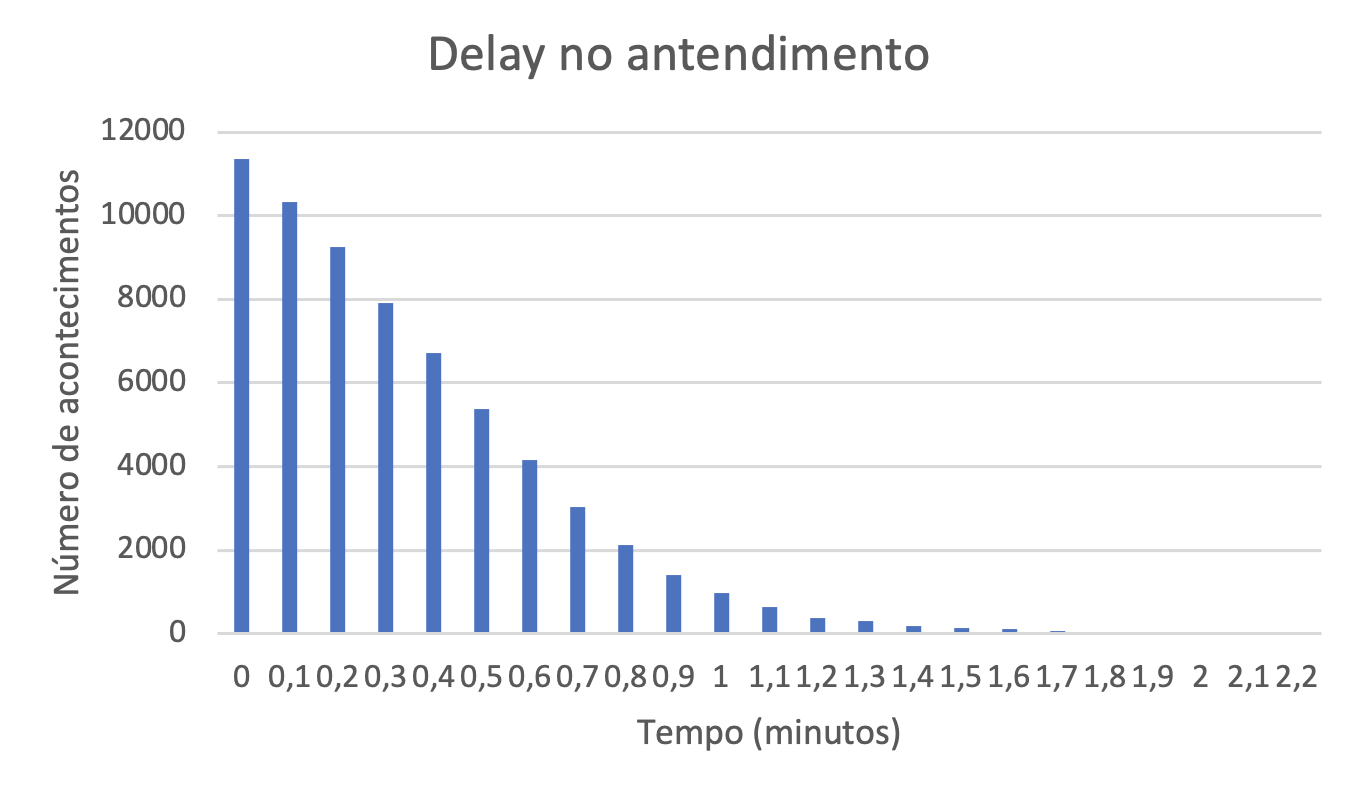
\includegraphics[width=\linewidth]{figs/intro/histo_delay.png}
    \caption{Distribuição dos delays no sistema}
    \label{fig:histo_delay}
    \end{subfigure}
    \hfill
    \begin{subfigure}[b]{0.5\textwidth}
        \centering
    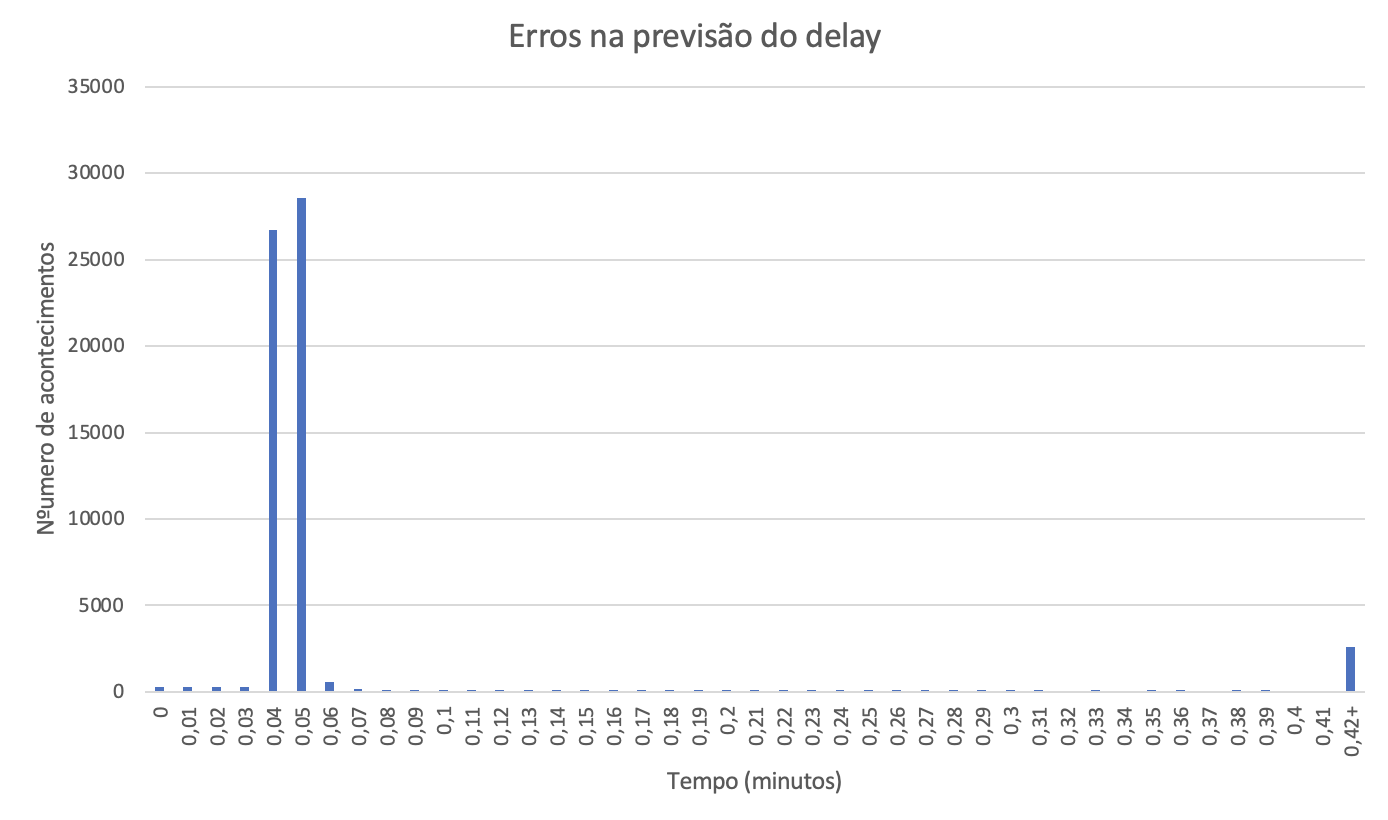
\includegraphics[width=\linewidth]{figs/intro/histo_erro.png}
    \caption{Distribuição do erro de previsão no sistema}
    \label{fig:histo_erro}
    \end{subfigure}
       \label{fig:histogramas}
\end{figure}

A distribuição dos dos \textit{Delays} aproxima-se de uma distribuição exponencial, pois este sistema é estável, ou seja, $\rho<1$.
Se $\rho>1$, esta distribuição seria crescente pois o tempo de espera iria aumentar com o tempo. Os delays 0 não estão representados.

Uma analíse do histograma dos erros indica que grande parte dos erros foi na ordem dos 0.04-0.06 segundos, que é sensivelmente o valor médio de atraso.
Mais uma vez, o facto do sistema ser estável fez com que os erros obtidos fossem da ordem da média.

\section*{Análise de Sensibilidade e Estimador}

\begin{figure}[H]
    \begin{floatrow}
    \ffigbox{%
    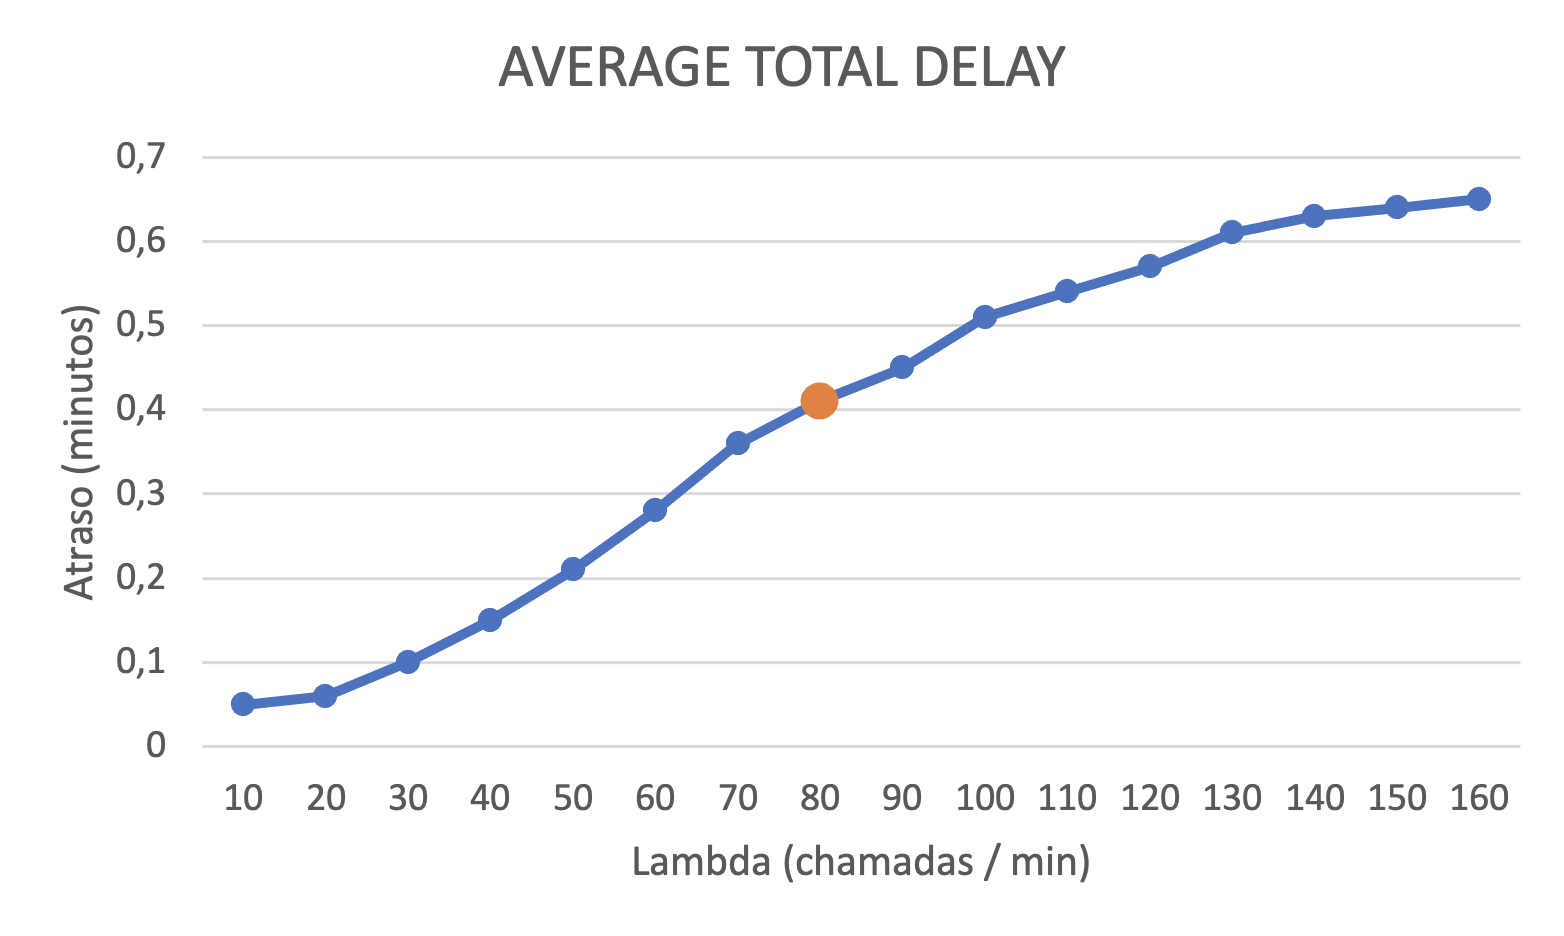
\includegraphics[width=.9\linewidth]{figs/intro/total_delay.png}
    }{%
    \caption{Total Delay time com variação da frequência de chegadas}
    }
    \capbtabbox{%
    \begin{tabular}{||c|c||} 
        \hline
        Intervalo de Confiança & 90\% \\
        \hline
        Número de Amostras & 30 \\
        \hline
        Graus de Liberdade & 29 \\
        \hline
        t (Student) & 1.6973 \\
        \hline
        Média & 0.410105 \\
        \hline
        Desvio Padrão & 0.005534535\\
        \hline
        Limite Inferior & 0.408389941 \\
        \hline
        Limite Superior & 0.411820059 \\
        \hline
       \end{tabular}
    }{%
    \caption{Estimador do Average Total Wait Time com intervalo de confiança de 90\% - 2 Tail}
    }
    \end{floatrow}
\end{figure}


A figura 4 mostra a relação entre a \textit{Arrival Rate} e o Atraso do sistema.
Observamos, como esperado, que o atraso tende para 0 à medida que se diminúi a \textit{Arrival Rate}.

À medida que o valor aumenta, o atraso tendo para um valor próximo de 0.65 minutos.
Isto deve-se ao facto da fila de espera ter tamanho limite.
O tempo que uma chamada tem que esperar se estiver no fim da fila não aumenta pois tem sempre o mesmo número de chamadas à sua frente.
O que aumenta é a probabilidade de perder a chamada. É deste modo de esperar este comportamento.

Também foi calculado um estimar para o Average Total Wait Time com base em 30 amostras do parâmetro.

